\documentclass[tikz,border=8pt]{standalone}
\usepackage[scaled]{helvet}
\renewcommand{\familydefault}{\sfdefault}
\usepackage[T1]{fontenc}
\usepackage[utf8]{inputenc}
\usepackage{tikz}
\usetikzlibrary{arrows.meta,positioning,calc}

\begin{document}
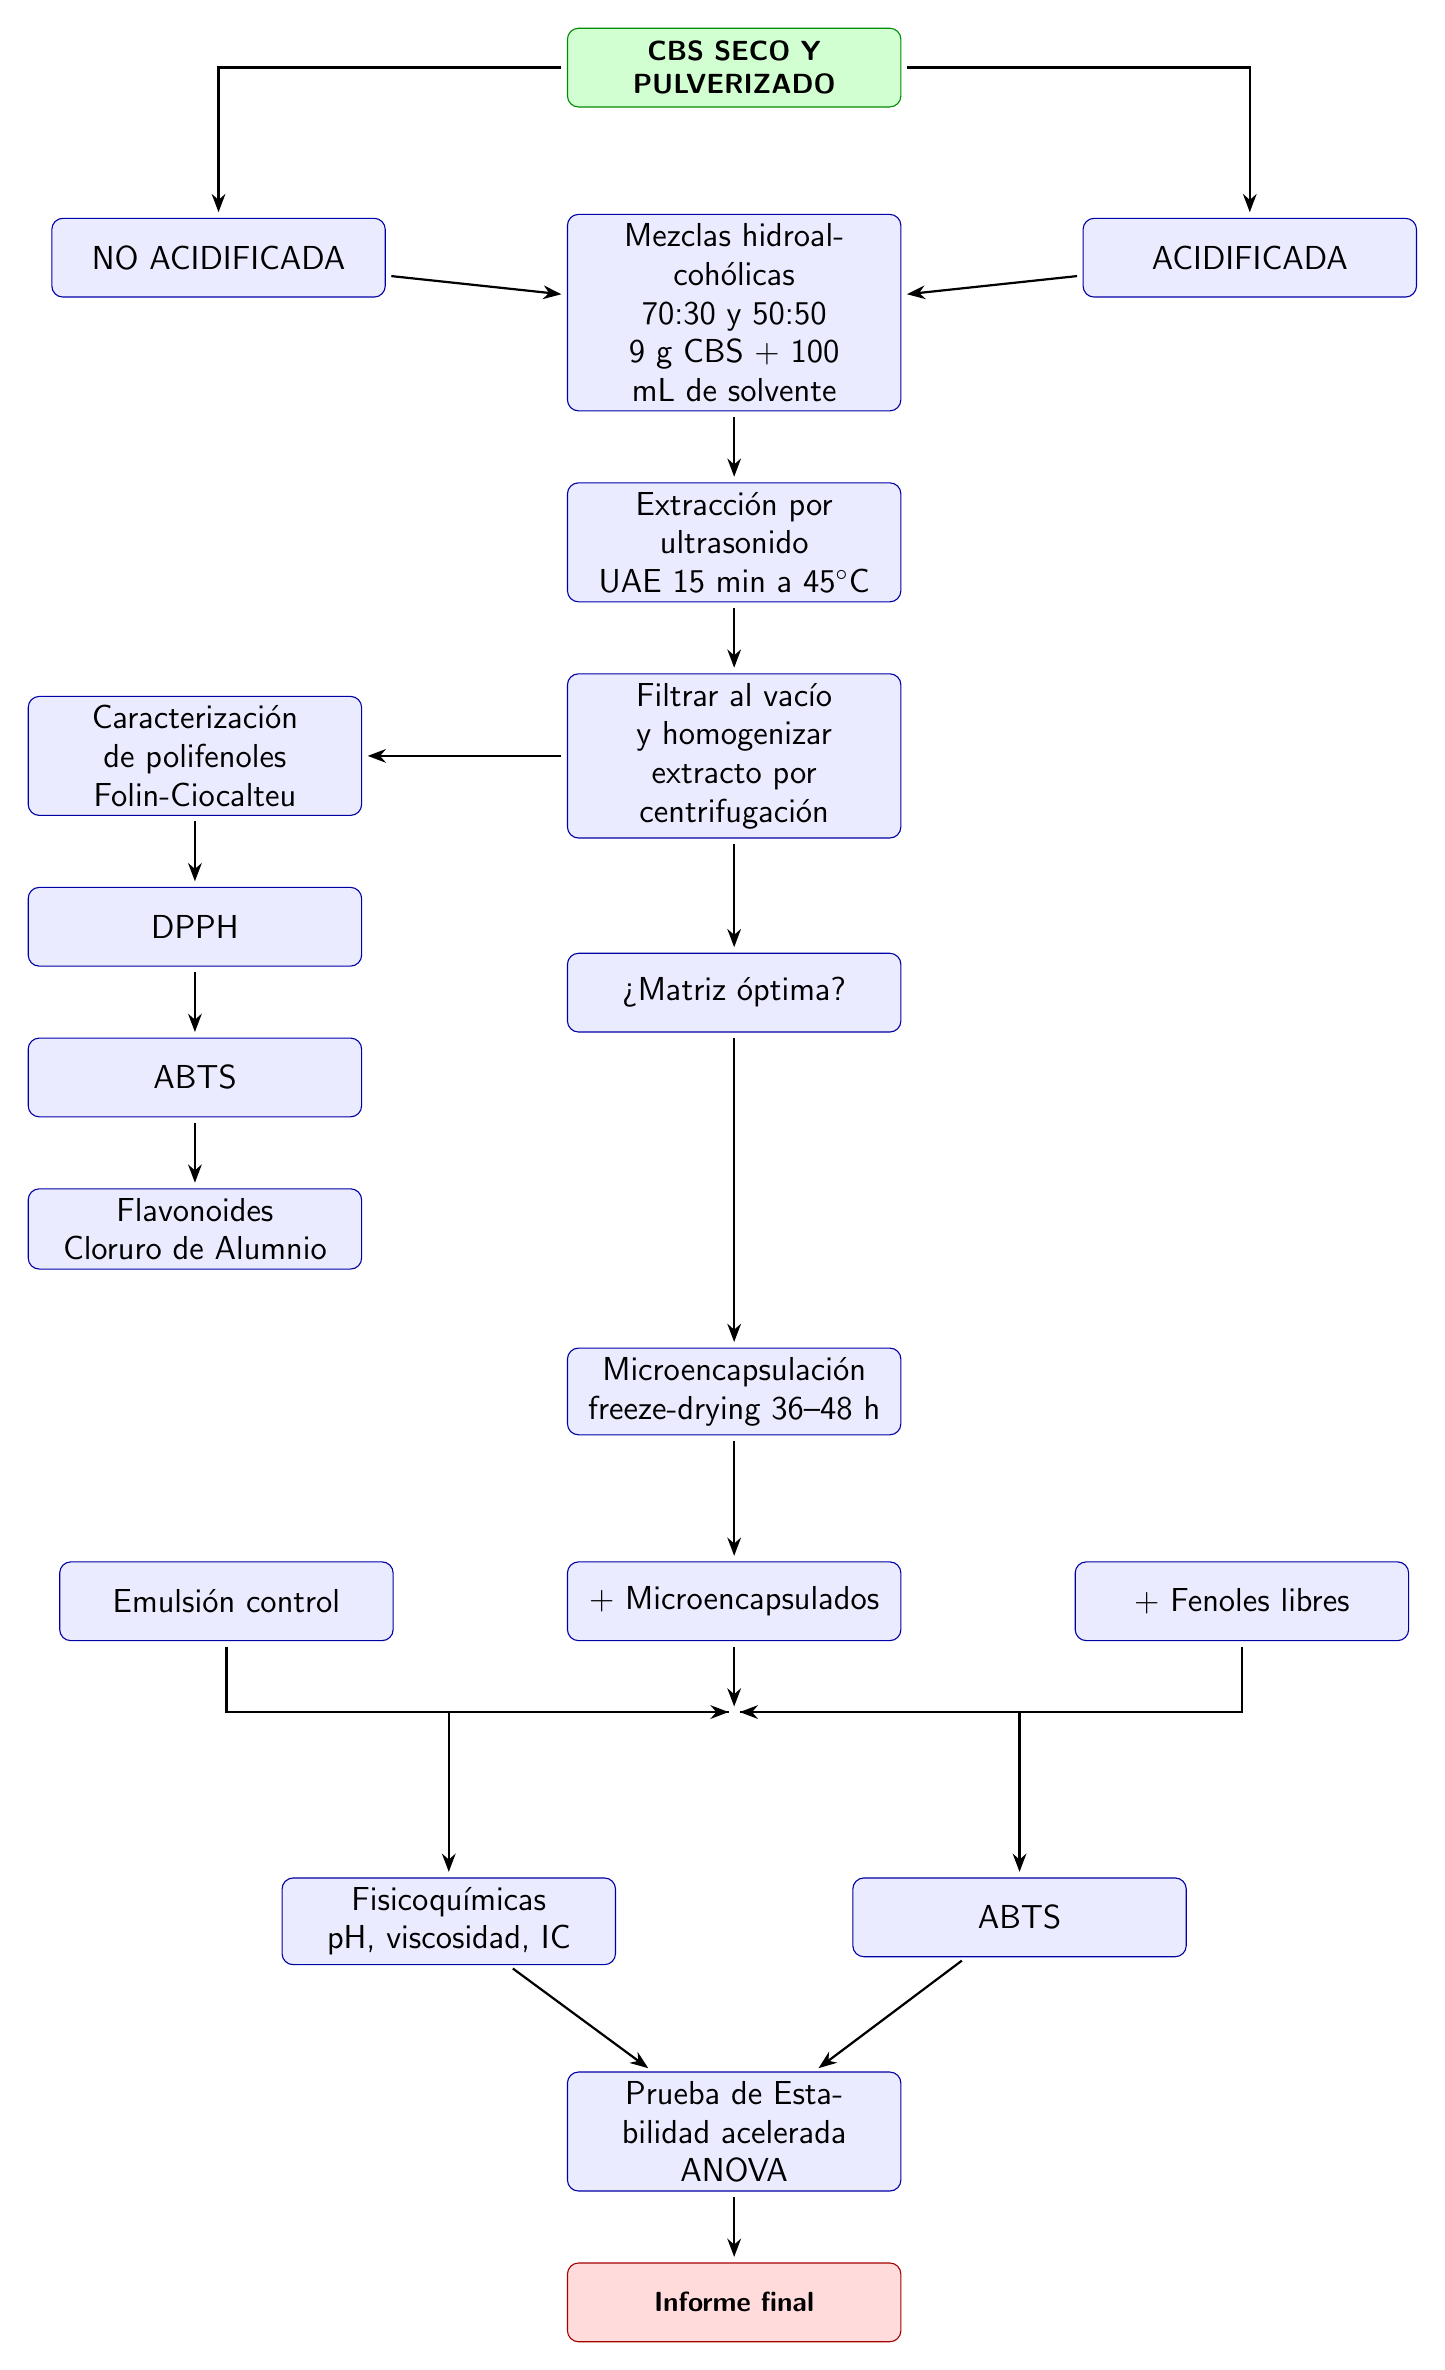
\begin{tikzpicture}[
  font=\fontsize{12}{14}\selectfont,
  node distance=0.9cm and 1.8cm,
  box/.style={
    rectangle, rounded corners,
    draw=blue!65!black, fill=blue!8,
    text width=4.0cm, minimum height=1.0cm, align=center
  },
  startbox/.style={
    box, draw=green!55!black, fill=green!18, font=\bfseries
  },
  endbox/.style={
    box, draw=red!65!black, fill=red!14, font=\bfseries
  },
  arrow/.style={
    ->, thick, >=Stealth, shorten <=2pt, shorten >=2pt
  }
]

% Main flow
\node[startbox] (cbs) {CBS SECO Y PULVERIZADO};

\node[box, below left=1.4cm and 2.3cm of cbs] (noac) {NO ACIDIFICADA};
\node[box, below right=1.4cm and 2.3cm of cbs] (ac) {ACIDIFICADA};

\node[box, below=1.35cm of cbs] (mezclas) {Mezclas hidroalcohólicas 70:30 y 50:50\\9 g CBS + 100 mL de solvente};
\node[box, below=of mezclas] (uae) {Extracción por ultrasonido\\UAE 15 min a 45$^\circ$C};
\node[box, below=of uae] (filtrar) {Filtrar al vacío y homogenizar\\extracto por centrifugación};

% Characterization branch
\node[box, left=2.6cm of filtrar] (fenoles) {Caracterización de polifenoles\\Folin-Ciocalteu};
\node[box, below=of fenoles] (dpph) {DPPH};
\node[box, below=of dpph] (abts1) {ABTS};
\node[box, below=of abts1] (flav) {Flavonoides\\Cloruro de Alumnio};

% Decision and microencapsulation
\node[box, below=1.45cm of filtrar] (mejor) {¿Matriz óptima?};

% MUCH LOWER than flav
\node[box, below=4.0cm of mejor] (freeze) {Microencapsulación\\freeze-drying 36--48 h};

% Emulsion boxes: SAME LEVEL, micro centered under freeze
\node[box, below left=1.6cm and 2.2cm of freeze] (control) {Emulsión control};
\node[box, below=1.6cm of freeze] (micro) {+ Microencapsulados};
\node[box, below right=1.6cm and 2.2cm of freeze] (libre) {+ Fenoles libres};

% Converging junction from the 3 emulsion boxes
\coordinate (merge) at ($(control.south)!0.5!(libre.south)+(0,-0.9cm)$);

% Two boxes below fed from converging line
\node[box, below left=2.1cm and 1.5cm of merge] (fisico) {Fisicoquímicas\\pH, viscosidad, IC};
\node[box, below right=2.1cm and 1.5cm of merge] (abts2) {ABTS};

% Stats below both
\coordinate (midfa) at ($(fisico.south)!0.5!(abts2.south)$);
\node[box, below=1.4cm of midfa] (stats) {Prueba de Estabilidad acelerada\\ANOVA};
\node[endbox, below=of stats] (final) {Informe final};

% Arrows
\draw[arrow] (cbs) -| (noac);
\draw[arrow] (cbs) -| (ac);
\draw[arrow] (noac) -- (mezclas);
\draw[arrow] (ac) -- (mezclas);

\draw[arrow] (mezclas) -- (uae);
\draw[arrow] (uae) -- (filtrar);

\draw[arrow] (filtrar) -- (fenoles);
\draw[arrow] (fenoles) -- (dpph);
\draw[arrow] (dpph) -- (abts1);
\draw[arrow] (abts1) -- (flav);

\draw[arrow] (filtrar) -- (mejor);
\draw[arrow] (mejor) -- (freeze);

% ONLY freeze -> micro
\draw[arrow] (freeze) -- (micro);

% Three emulsion boxes -> converging line (orthogonal, no curves)
\draw[arrow] (control) |- (merge);
\draw[arrow] (micro) -- (merge);
\draw[arrow] (libre) |- (merge);

% Converging line -> fisico and abts2
\draw[arrow] (merge) -| (fisico.north);
\draw[arrow] (merge) -| (abts2.north);

% fisico and abts2 -> stats
\draw[arrow] (fisico) -- (stats);
\draw[arrow] (abts2) -- (stats);

\draw[arrow] (stats) -- (final);

\end{tikzpicture}
\end{document}